\chapter{Literature review}


This chapter provides a review of the relevent literature separated into 3 parts. First is literature revelent to the \emph{DISPLIB}. Second are the most revelevant resources inspiring the heuristic or providing key theoretical ideas. Third is an overview of selected state of the art in scheduling optimization.

\section{DISPLIB}

As the main goal of this thesis is to make a heuristic that solves instances from the \emph{DISPLIB} library, we provide a review of the introductory paper as well as a description of the competiton winning solutions.

\subsection{Problem and library}
The train dispatching problem (TDP) which this thesis is working with is presented in \emph{DISPLIB: A library of train dispatching problems } \cite{kloster2025displiblibrarytraindispatching} alongside the collection of instances which can be used to benchmark this problem. This provides an imporant step for the subfield of train dispatching optimization - a unified problem format and real-life data to be used for benchmarking. The instances and competition results can be accesed from~\url{https://displib.github.io/}.

\blockcquote{kloster2025displiblibrarytraindispatching}{
	... each study (on train scheduling) is typically tightly connected with a specific industrial use case. Code and data are seldom shared publicly. This fact hinders reproducibility, and has led to a proliferation of papers describing algorithms for more or less compatible problem definitions, without any real opportunity for readers to assess their relative performance. Inspired by the successful communities around MILP, SAT, TSP, VRP, etc., we introduce a common problem definition and file format, \emph{DISPLIB}, which captures all the main	features of train re-routing and re-scheduling.
}

The instances are published with best known solutions (assumed with unlimited time), unfortunatelly for the 10 minute computation time limit only the competition team rankings are presented, without overview of the actual solutions.

\subsection{Competition and solutions}
Part of the presentation of \emph{DISPLIB} was also the anouncement of the competition for optimization using this library. The competition concluded at the Optimization and Decision Science Conference (ODS) 2025 where they presented the winners. Unfortunatelly the materials for the solutions are not available and only one team wrote a paper about their solution. Still, we find essential to provide the reader with the description for other solutions, so the limited information from the book of abstracts for the ODS 2025 \cite{ods2025bookofabstracts} is summarized.

The first place went to Carolin Scholl and Luka Stärk (DB Systel GmbH). Their solution is based on branch and bound inspired by Monte Carlo Tree Search \cite{DARIANO2007643}, prioritizing not only lower bound improvement but also search for feasible solutions. In each step of the tree they resolve the chronologacally first conflict either by setting precedence to either of the trains on the conflicting resources or by rerouting either train if possible. This is a bottom-up approach, only adding the necessary constrains for current conflicts.

The second place went to Openbus team (ETH Zürich) which published a description of their solution in \emph{Handling Conflicts in Microscopic Railway Timetabling at Scale: A Hybrid Approach}\footnote{This paper is not officially published, only a pre-print was available.} \cite{Dubach2025handling}. Their solution utilizes 2 distinct solvers which run in parallel. First one is a Logic-Based Benders Decomposition (LBBD) procedure \cite{Leutwiler2022logic} where a master mixed-integer programing (MIP) problem performs a selection of current available paths, slave satisfiability modulo theory (SMT) solver creates a feasible time table if possible (without conflicts) and a subproblem detects conflicts and adds them SMT solver, which in turn adds cuts to the master problem to maintain feasiblity. Figure \ref{fig:openbus_lbbd} show the diagram of the solver as presented in their poster. Second solver uses a simpler MIP representation which iteratively relaxes the bounds for conflicing resources and tightens the bounds for non-conflicing resources converging to a feasible solution. Both of these solvers use a bottom-up approach, after a bound tightening procedure is applied globally. The authors argue that both of these solvers exploit different instance structures and share their bounds to improve convergence.

\begin{figure}[htbp!]
\caption{Openbus DISPLIB competition poster}
\label{fig:openbus_lbbd}
\begin{center}
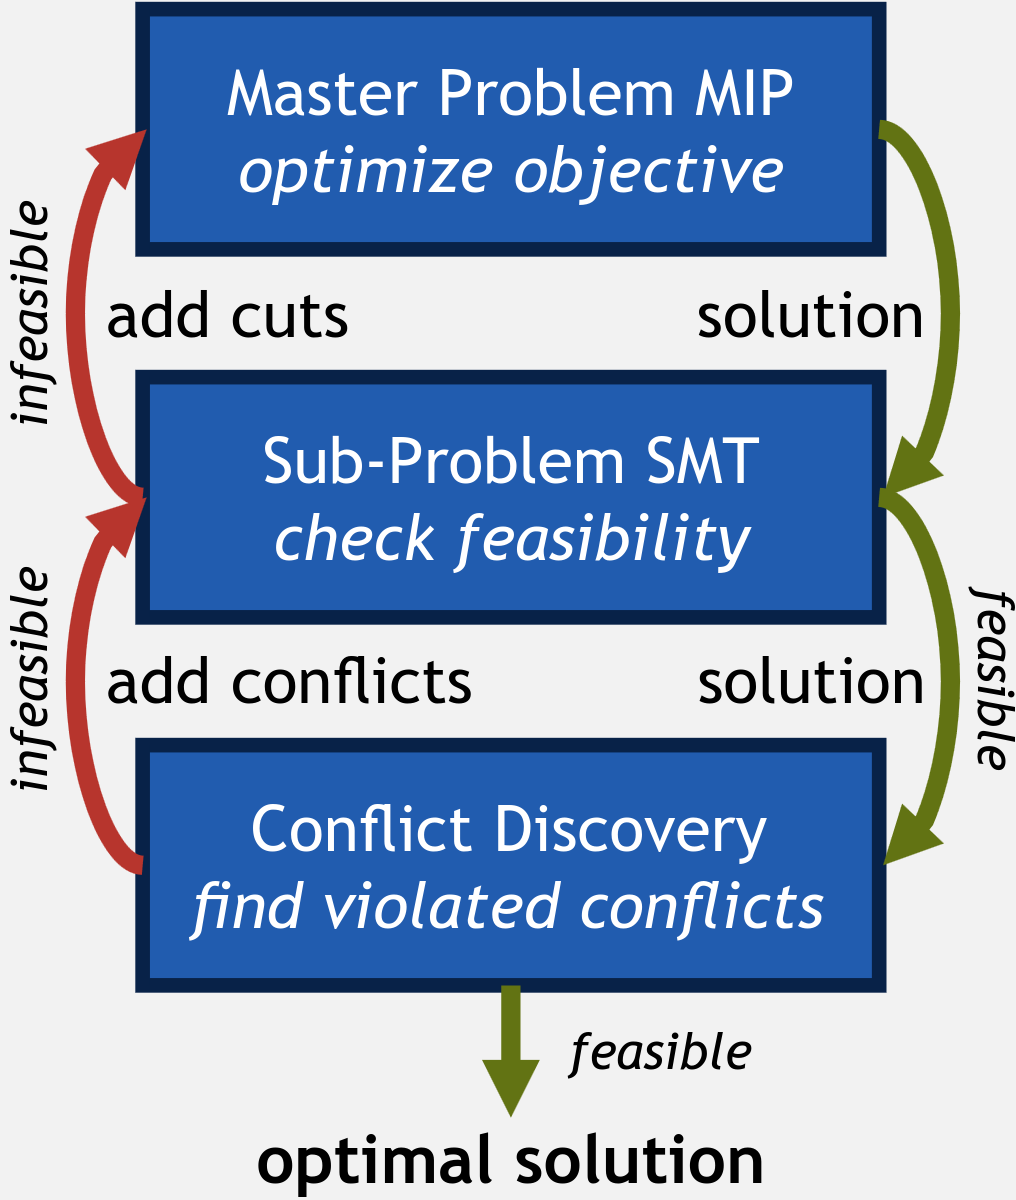
\includegraphics[width=.525\textwidth]{img/openbus_lbbd.png}
\end{center}

\footnotesize \textit{Source:} ETH Zürich Research Collection \cite{Dubach2025poster}
\end{figure}

The third place went to Venislav Steliyanov Varbanov (independent). This solution also uses an MIP model with a decomposition to reduce the number of time variables - this idea is also used by the heuristic in this thesis, inspired by the provided description. After this aggregation of time variables, the conflicts are again resolved sequentially, similarly to the other 2 solutions.

We can see that while the winning solutions may differ in their model representation and optimization approach, and 2 of them use a certain level of aggregation, they have one thing in common - they resolve the conflicts sequentially and thus they only need to consider the conflicts that arise in the current partial solution and therefore the number of constrains and variables necessary to prevent the conflicts stays limited.

\section{Theory and heuristics}

While the \emph{DISPLIB} winning solutions provided us with the ideas of aggregation of variables and combining conflict resolutions, it provided very little on the actual implementation. This section descibes the relevant sources to explain the necessary theory to model the problem effectively.

Referenced by the winning solution is \emph{A Branch and Bound Algorithm for Scheduling Trains in a Railway Network} \cite{DARIANO2007643}. It uses an alternative graph formulation for the train scheduling problem. With this representation we can model resouce conflicts with alternative precedence arcs. It also describes the idea of inferred selection, meaning that by choosing one precence alternative for a resource implies selection on another resources (the alternative is forbidden as it would produce an infeasible solution).

\emph{Job-shop Scheduling with Blocking and No-wait Constraints} \cite{MASCIS2002498} introduces the alternative graph concept as a generalization of the disjunctive graph \cite{roy1964problemes}. The alternative graph is used to formulate a model for the blocking job-shop problem (BJSP) that is closely related to TDP.

\emph{Improving Real-Time Train Dispatching: Models, Algorithms and Applications.} \cite[p. 84-85]{dariano2008improving} provides static implication rules for the alternative graph representation that can be used for inferred selection based on the structure of TDP.

\emph{Railway scheduling problems and their decomposition} \cite{Strotmann2007} is thesis that show decomposition techniques that inspired the decomposition used in this thesis to split the global problem into small subgraphs using border operations and a global synchronizer to merge the solution from these subgraphs and deal with potention conflicts.

\section{State of the art}
Because the description of the solutions that are directly connected to this thesis is limited, we provide the reader with an overview of the recent state of the art solutions for closely related problems in train dispatching and scheduling.

\emph{Optimizing train dispatching for the Union Pacific Railroad}~\cite{boccia2025optimizing} presents an automated dispatching system that is in use on a real rail network. It uses a decomposition of the problem and global synchronizer to resolve conflict. It is a prime example how optimization can improve real-life solutions.

\emph{A Branch-and-Cut Algorithm for Scheduling Train Platoons in Urban Rail Networks}~\cite{chai2024branch} describes a mixed-integer linear problem (MILP) for scheduling of train platoons, problem where different vehicles are flexibly and dynamically coupled and decoupled.

Authors in \emph{Decentralised Multi-Agent Coordination for Real-Time Railway Traffic Management} \cite{damato2025decentralised} propose the use of another emerging idea - instead of central or area based decomposition schedulers, trains cooperate as separate agents to prevent conflicts and achieve efficient scheduling. This decentralized nature of cooperation has already been used on drone related problems with success \cite{HertJINTHW_paper}.


